\documentclass[../../Main/Appunti Fisica.tex]{subfiles}
\begin{document}
Si consideri la figura di seguito riportata, rappresentante un campo magnetico uniforme perpendicolare ad una superficie.
\begin{figure}[!h]
    \centering
    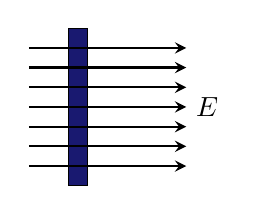
\begin{tikzpicture}[scale = 1, every node/.style={scale=1}]
        % Surface crossed by the electric field
        \draw [fill = MidnightBlue] (0, 0) rectangle (0.25, -2);

        % Electric field lines
        \foreach \i in {1, 2, ..., 7}{
                \draw [-stealth, thick] (-0.5, -0.25 * \i) -- (1.5, -0.25 * \i);
            }

        \node [anchor = west] at (1.5, -1) {\(\va{E}\)};
    \end{tikzpicture}
    \caption{Superficie attraversata da campo elettrico.}
    \label{fig:12}
\end{figure}

Si definisce \textit{flusso elettrico} il numero di linee di campo che attraversano una superficie.
Più precisamente questi si definisce come
\[
    \Phi_{E} \equiv \vb{E}A
\]
Se la superficie \(A\) non è perpendicolare al campo, questa formerà un certo angolo \(\theta\) con \(\va{E}\).
Più in generale il flusso elettrico è definito come
\[
    \Phi_{E} \equiv \vb{E} A \cos \theta
\]

Si consideri ora il caso in cui \(\va{E}\) non sia uniforme.
Se si considera una superficie \(A\) divisa in tante piccole aree \(\Delta \va{A_{i}}\), segue che ciascuna sortirà un campo \(\va{E_{i}}\) generalmente uniforme.
Dunque il flusso su ogni elemento sarà
\[
    \Delta \Phi_{E} = \vb{E_{i}} \Delta A_{i} \cos \theta
\]
%
Da ciò, integrando, il flusso elettrico totale sarà
\begin{equation}\label{eq:14}
    \Phi_{E} = \oint{}{}{\va{E} \cdot}{\va{A}}
\end{equation}
\end{document}
\clearpage